\documentclass[11pt]{article}
\usepackage[margin=0.9in]{geometry}
\usepackage[T1]{fontenc}
\usepackage{lmodern}
\usepackage{amsmath,amssymb}
\usepackage{booktabs,graphicx}
\usepackage{float}
\usepackage{xcolor}
\usepackage{tikz}
\usetikzlibrary{arrows.meta,positioning,fit,calc}
\usepackage[hidelinks]{hyperref}
\hypersetup{
  pdftitle={DiagPriv: Preserving Diagnostic Structure While Reducing Sensitive Data Exposure in LLM Root-Cause Analysis},
  pdfauthor={Keshav Likhar, Harsh Mandalgi, Mohit Chaturvedi},
  pdfsubject={Editorial revision v1.1 of the DiagPriv development-stage preprint},
  pdfkeywords={root-cause analysis, large language models, privacy-oriented transformation, diagnostic invariants}
}
\usepackage{microtype}
\setlength{\parskip}{0.25em}
\setlength{\parindent}{1em}
\title{DiagPriv: Preserving Diagnostic Structure While Reducing Sensitive Data Exposure in LLM Root-Cause Analysis}
\author{
Keshav Likhar\thanks{Corresponding author: \href{mailto:keshavlikhar007@gmail.com}{keshavlikhar007@gmail.com}.}\thanks{All authors contributed equally to this work.}\\
\small Independent Researcher, Boise, Idaho, USA\\
\small ORCID: \href{https://orcid.org/0009-0000-1473-8274}{0009-0000-1473-8274}
\and
Harsh Mandalgi\\
\small Independent Researcher, Bengaluru, India\\
\small ORCID: \href{https://orcid.org/0009-0000-9956-3636}{0009-0000-9956-3636}
\and
Mohit Chaturvedi\\
\small Independent Researcher, Buffalo, New York, USA\\
\small ORCID: \href{https://orcid.org/0009-0001-7496-1504}{0009-0001-7496-1504}
}
\date{}

\begin{document}
\maketitle
\begin{abstract}
Operational evidence can help an external large language model (LLM) find a
failure cause. The same evidence can reveal identifiers and time data that the
model does not need. We test transformations that hide selected values but
keep relations needed for root-cause analysis (RCA). Three synthetic incident
families require identifier linkage, identifier shape, or temporal order.
The tests compare redaction, three types of pseudonyms, relative time, and
temporal ablation. A separate exposure vector measures the information that
remains visible. It is not an anonymity score. Development results suggest
that task-specific structure can affect RCA. However, the study uses few
synthetic cases, one model family, and no held-out evaluation. It gives no
formal privacy guarantee.
\end{abstract}

\section{Introduction}
Engineers use logs, traces, and operational records to investigate outages.
LLM-based RCA systems also use this evidence
\cite{ahmed2023recommending,chen2024automatic,wang2024rcagent,xu2025openrca}.
The records can contain customer IDs, account links, request history, time
data, and secrets. Sending all records to an external model can expose data
that the task does not need. A generic redaction marker can also remove the
joins that explain the failure. A stable pseudonym keeps joins, but it can
expose frequency and linkage. Thus, the important question is which relations
remain visible after a transformation.

DiagPriv names these task-required relations \emph{diagnostic invariants}.
Examples include repeated request identity, identifier shape, and event order.
The study measures both RCA utility and information exposure. It does not
claim that transformed data is anonymous.

Three deterministic synthetic families test different dependencies.
Incident 001 needs identifier linkage. Incident 002 needs identifier shape.
Incident 003 v3 needs temporal order and overlap. Table~\ref{tab:families}
summarizes the designs.
\begin{table}[H]
\centering
\small
\resizebox{\textwidth}{!}{%
\begin{tabular}{llll}
\toprule
Family & Observed problem & Key invariant & Mechanism contrast \\
\midrule
001 & Duplicate payment effect & Identifier equality and cross-source linkage & Timeout, re-arrival, missing idempotency \\
002 & Missing provisioning effect & External-reference format and shape & Malformed reference, exact lookup miss \\
003 v3 & Premature compensation / twin & Deadline order and interval overlap & Overlapping execution versus serialized invalid transition \\
\bottomrule
\end{tabular}%
}
\caption{Three synthetic incident families and their intended diagnostic dependencies.}
\label{tab:families}
\end{table}


Prior work covers task-aware anonymization and evidence-grounded RCA
\cite{loiseau2025taueval,loiseau2026adaptive,wang2026cloudopsbench}. This work
adds a bounded evaluation design. It separates the oracle from the ModelView,
compares fixed transformations on matched development cases, reports an
exposure vector, and scores cited evidence separately from RCA labels. It does
not implement an automatic transformation selector.

\section*{Glossary}
\begin{description}
\small
\item[Diagnostic invariant.] A relation in visible evidence that an RCA task
needs, such as two records that contain the same request ID.
\item[Exposure.] Information that remains visible in the exact data sent to
the model. Exposure is not the same as re-identification risk.
\item[HMAC.] A keyed hash function. DiagPriv uses it to make stable opaque
identifiers. The key stays inside the trusted system.
\item[ModelView.] The question and evidence that the external model receives.
It excludes oracle answers and transformation secrets.
\item[Oracle.] The frozen reference answer used for scoring.
\item[Pseudonymization.] Replacement of a value with another value. A stable
pseudonym can preserve equality and frequency.
\item[RCA.] Root-cause analysis: the process that identifies why an incident
occurred.
\item[Temporal ablation.] A destructive control that removes usable time
relations from the ModelView.
\end{description}

\section{Motivation and Threat Model}
\label{sec:threat}
The trusted system contains the data sources and the transformation layer.
The external model receives only a question and a transformed ModelView.
The provider is honest-but-curious: it performs the task, but it should not
receive unnecessary data. This model does not cover a compromised provider or
an attacker who controls the trusted host.

\begin{figure}[H]
\centering
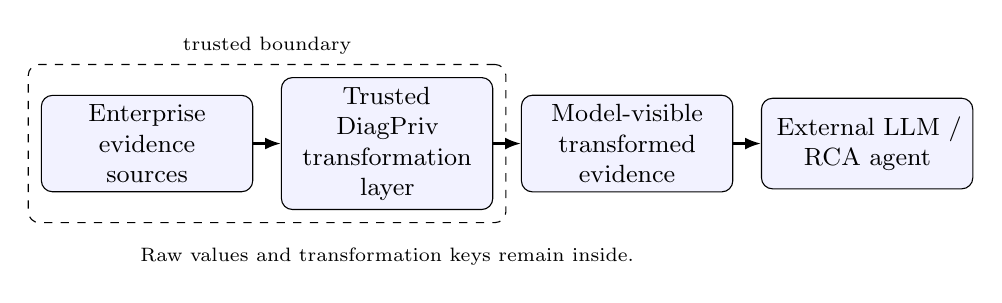
\begin{tikzpicture}[
  node distance=0.35cm,
  box/.style={draw,rounded corners,minimum height=1.15cm,text width=2.45cm,
              align=center,fill=blue!5,font=\small},
  arrow/.style={-{Latex[length=2mm]},thick}
]
\node[box] (source) {Enterprise evidence\\sources};
\node[box,right=of source] (transform) {Trusted DiagPriv\\transformation layer};
\node[box,right=of transform] (view) {Model-visible\\transformed evidence};
\node[box,right=of view] (model) {External LLM /\\RCA agent};
\draw[arrow] (source) -- (transform);
\draw[arrow] (transform) -- (view);
\draw[arrow] (view) -- (model);
\node[draw,dashed,rounded corners,fit=(source)(transform),inner sep=0.16cm,
      label={[font=\scriptsize]above:trusted boundary}] {};
\node[font=\scriptsize,align=center,below=0.36cm of transform]
      {Raw values and transformation keys remain inside.};
\end{tikzpicture}
\caption{The intended data boundary. The study measures the released
representation. It does not measure provider retention.}
\label{fig:architecture}
\end{figure}

Protected assets include identity, linkable IDs, original format, timestamps,
and field relations. A declared \texttt{secret} or \texttt{never\_release}
literal must not occur in the released view. Synthetic tests enforce this
rule. No current development field has that label. Record counts and
unannotated timestamps can still remain visible.

This threat model does not replace access control. It does not measure
re-identification, provider retention, prompt injection, malicious agents, or
legal compliance.

\section{Problem Formulation and Diagnostic Invariants}
\label{sec:formulation}
Let $D$ denote raw operational evidence, $Q$ the troubleshooting question,
and $A$ the field policy. A condition $T_c$ produces released evidence
$D'_c=T_c(D;A)$. The model receives only $(Q,D'_c)$ and returns
\[
R=(o,t,a,m,k),
\]
where the fields are outcome, trigger, action, mechanism, and owning
component. Exact RCA requires all five fields to match the frozen oracle.

For task $Q$, $I_Q=\{i_1,\ldots,i_n\}$ is the set of declared diagnostic
relations. An audit marks each relation as genuinely preserved, broken,
preserved by degenerate collapse, or intentionally not preserved. This audit
does not prove that a model will use the relation correctly.

The objective is to keep required relations and reduce unnecessary release:
\[
\text{seek }T_c\text{ such that }i_j(D,Q)\text{ remains assessable in }D'_c
\quad\text{for essential }i_j.
\]
Utility and exposure are separate vectors, not one score. Incident 001 needs
request equality but not a customer name. Incident 002 needs reference shape
but not its literal characters. Incident 003 needs relative order and overlap
but not the calendar date.

\section{DiagPriv Transformation Framework}
\label{sec:framework}
The implementation keeps benchmark construction, transformations, prompt
rendering, provider invocation, and oracle scoring separate. A generator
produces an \texttt{Incident} with model-visible records and oracle-only
labels, privacy annotations, expected evidence, and invariant definitions.
Transformations begin from \texttt{Incident.model\_view()} and return a new
\texttt{ModelView}; neither an oracle answer nor the HMAC key is serialized
into the model request. A versioned condition and hash identify each
representation. The fixed baselines below isolate different preservation
choices rather than claiming to be interchangeable security mechanisms.

\paragraph{Redaction and deterministic pseudonyms.}
\texttt{redaction-v1} replaces annotated values with field-class
placeholders. It hides raw literal identity but can collapse distinct
entities and destroy meaningful joins. \texttt{hmac-v1} uses keyed,
namespace-separated HMAC-SHA-256 identifiers; it preserves deterministic
equality within declared namespaces, including selected cross-source joins,
while retaining frequency and linkability. Its operational key is external
to prompts and artifacts. The privacy-exposure analysis uses a separate
public synthetic test-only key and makes no operational key-compromise claim.
\texttt{tokenization-v1} assigns short, deterministic, ephemeral tokens from
a mapping over the complete view. Its mapping is reproducible for the same
input population but is neither a persistent production vault nor
guaranteed globally stable across independently transformed candidate sets.
Both methods can expose candidate-set or frequency information even when raw
values disappear.

\subsubsection*{Shape and time}
\texttt{format-preserving-v1} is deterministic format/constraint-preserving
pseudonymization: it retains measured length, separator positions, and
character classes while changing literal values. It is \emph{not}
cryptographic format-preserving encryption. \texttt{relative-time-v1}
converts annotated timestamps to incident-local millisecond offsets,
removing the original absolute representation but keeping equality,
ordering, gaps, durations, and overlap. Exact offsets could reconstruct
absolute times given an external anchor. \texttt{temporal-ablation-v1}
replaces annotated timestamps with non-temporal markers and removes log-order
leakage; it is a destructive causal control, not an optimal privacy method.
In Incident 001 and 002 the scalar methods leave \emph{unannotated}
timestamps unchanged, a limit measured explicitly below.

These conditions are versioned; no transformation was retuned after observing
the results reported here. The broader DiagPriv ambition is to choose a
least-exposing condition that preserves the declared essential relations for
the task. This draft evaluates the premise with fixed baselines. It does not
present an implemented task-aware planner or an automatic guarantee of
minimal disclosure.

\section{Benchmark and Evaluation Methodology}
\label{sec:method}
DiagBench constructs fictional operational records from deterministic
generators. Each incident separates a complete oracle-bearing object from
the exclusive model-facing question, structured rows, and logs. Evidence
elements have stable visible IDs; scorer and invariant code may consult
oracle references offline, but the prompt cannot. Construction audits check
that the intended causal relation is visible, nuisance variation is present,
and prohibited shortcuts do not separate the oracle cases. This makes a
generator test an implementation/construction check, not evidence that a
human or model finds the case realistic or difficult.

The experiments use frozen development selections. Incident 001 uses
seeds 1000--1004 for the privacy comparison with GPT-5.6 Luna; its earlier
raw-only 2000--2009 validation observation is reported separately.
Incident 002 uses the first ascending development seed for each of six
hidden defect classes (1000, 1001, 1003, 1004, 1005, 1017), not seeds chosen
for model performance. Its GPT-5.6 Sol comparison has three logical trials
per seed-condition. Incident 003 v3 uses four constructions selected by a
frozen content-independent rule (1319, 1299, 1387, 1222), each with target
and temporal-twin queries over the same evidence. The current paper has no
final held-out evaluation. It does not access new validation cases.

The model-facing prompt fixes a canonical output vocabulary, demands a
five-field RCA, an explanation, and supporting evidence IDs. Incidents 001
and 002 use \texttt{raw-rca-v2}, \texttt{rca-taxonomy-v2}, and
\texttt{raw-rca-scorer-v2}. Incident 003 v3 uses the separately frozen v3
versions. Provider requests use medium reasoning and omit temperature;
the originally intended Luna zero-temperature field was rejected by that
provider configuration, whereas Sol omission preserves the matched
protocol without implying Sol rejection. Trial identity, prompt-template
hash, exact rendered model-input hash, transformation provenance, scoring
versions, and response status are recorded as available. Incorrect
diagnoses are not silently retried. Infrastructure failures are retained
as missing model responses, not scored as wrong diagnoses.

We report exact five-dimensional RCA, individual dimensions, and, for
Incident 003, whether both queried roles in a construction receive their
correct mechanisms. Evidence support is not inferred from label correctness:
it is evaluated separately as described in Section~\ref{sec:evidence}.
Representation exposure is a third separate analysis over the exact released
\texttt{ModelView}, not over hidden generator state. Paired comparisons reuse
the same construction under matched conditions; Incident 003's two roles
share the same evidence but differ in their subject-specific question.

The three Incident 003 provider stages were authorized and executed
separately under frozen inputs. Their ignored local JSONL artifacts have
these exact SHA-256 identities (raw, relative-time, ablation):
\begin{center}
\scriptsize
\begin{tabular}{ll}
\toprule
Stage & Frozen result SHA-256 \\
\midrule
Raw & \texttt{b5b567e5966047bc075cdfa2287b13a700e83eb870f2366ee0291dac595505a2} \\
Relative time & \texttt{f020511aeb497eab8c4ca5da4487ed87e20c6fe5e8b37a56613eb521297536e4} \\
Temporal ablation & \texttt{40d48f58f95b9bf837fa75a6a13209f6d00c6bbedca8c24d90ddb0927e1bb55a} \\
\bottomrule
\end{tabular}
\end{center}
The repository contains deterministic generators, transformations, scorers,
configs, protocol and aggregate-result documents, and the privacy-exposure
artifact. This tracked material provides Level-1 reproducibility for software,
deterministic analyses, aggregate tables, and frozen artifact identities.
The separate frozen-artifact manifest and offline verifier define a
provenance-safe design for authorized exact-byte verification, but no private
provider-observation archive is currently provisioned and no public
observation-level release exists. The provider JSONLs therefore remain
ignored local records: aggregate-table regeneration is available now, while
independent inspection of the exact historical provider responses is not.

\section{Incident-Family Design}
\label{sec:families}
\paragraph{Incident 001: duplicate payment.}
A timeout precedes re-arrival of one logical request. The executor lacks an
effective idempotency control and records two successful effects. The cause is
missing or ineffective idempotency in the operation executor. Required
structure includes same-request linkage, two distinct effects, success states,
and event order. The literal customer identity is not required.

\paragraph{Incident 002: malformed external reference.}
A provisioning request has an unexpected reference shape. An exact lookup
misses, and no effect occurs because validation or normalization is
inadequate. Controls make lookup miss and latency alone insufficient. The
target's deviation from a healthy shape is the intended clue. A hidden
\texttt{leading\_zero\_loss} cause is visible only as deletion at the leading
position of a numeric run. The visible data does not reveal the missing digit.

\paragraph{Incident 003 v3: temporal causal isolation.}
The target execution overlaps compensation after a deadline. Correct
serialization would prevent the outcome, so the mechanism is incorrect
concurrency control. The temporal twin has the same
non-temporal signatures. Its effect completes before the deadline, and later
compensation is an invalid serialized transition. Its mechanism is
incorrect state transition. Offline audits found matching
non-temporal projections across 200 development constructions.

\begin{figure}[H]
\centering
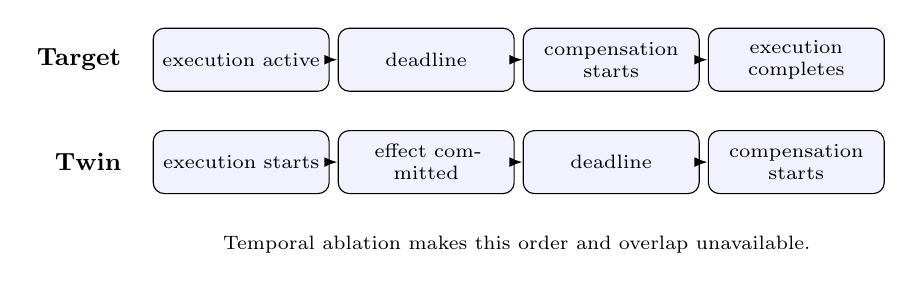
\begin{tikzpicture}[
  eventbox/.style={draw,rounded corners,fill=blue!5,font=\scriptsize,
               text width=2.0cm,align=center,minimum height=0.8cm},
  label/.style={font=\small\bfseries,anchor=east},
  flow/.style={-{Latex[length=1.7mm]},thick}
]
\node[label] at (0,2.2) {Target};
\node[eventbox] (ta) at (1.4,2.2) {execution active};
\node[eventbox] (tb) at (3.75,2.2) {deadline};
\node[eventbox] (tc) at (6.1,2.2) {compensation starts};
\node[eventbox] (td) at (8.45,2.2) {execution completes};
\draw[flow] (ta)--(tb);\draw[flow] (tb)--(tc);\draw[flow] (tc)--(td);
\node[label] at (0,0.9) {Twin};
\node[eventbox] (wa) at (1.4,0.9) {execution starts};
\node[eventbox] (wb) at (3.75,0.9) {effect committed};
\node[eventbox] (wc) at (6.1,0.9) {deadline};
\node[eventbox] (wd) at (8.45,0.9) {compensation starts};
\draw[flow] (wa)--(wb);\draw[flow] (wb)--(wc);\draw[flow] (wc)--(wd);
\node[font=\scriptsize,align=center] at (4.9,-0.15)
{Temporal ablation makes this order and overlap unavailable.};
\end{tikzpicture}
\caption{Incident 003 mechanism contrast. The diagram is schematic.}
\label{fig:temporal-isolation}
\end{figure}

\section{Experimental Results}
\label{sec:results}
All numerical comparisons here are descriptive observations on selected
synthetic development instances. They do not establish statistical
significance, population-level effect sizes, or a universal transformation
ranking. Table~\ref{tab:utility} reports the first two incident families
with their distinct model and repetition protocols.
\begin{table}[H]
\centering
\small
\resizebox{\textwidth}{!}{%
\begin{tabular}{llrrrrrr}
\toprule
Family & Condition & Literal & Equal & Unequal & Frequency & Cross-source & Shape \\
\midrule
001 & Raw & 476/476 & 559/559 & 3459/3459 & 20/20 & 326/326 & 476/476 \\
001 & Redaction & 0/476 & 233/559 & 1709/3459 & 0/20 & 0/326 & 0/476 \\
001 & HMAC & 0/476 & 509/559 & 3459/3459 & 15/20 & 276/326 & 0/476 \\
001 & Tokenization & 0/476 & 509/559 & 3459/3459 & 15/20 & 276/326 & 0/476 \\
001 & Format-preserving & 0/476 & 509/559 & 3459/3459 & 15/20 & 276/326 & 476/476 \\
002 & Raw & 190/190 & 300/300 & 2656/2656 & 6/6 & 248/248 & 190/190 \\
002 & Redaction & 0/190 & 52/300 & 1680/2656 & 0/6 & 0/248 & 0/190 \\
002 & HMAC & 0/190 & 300/300 & 2656/2656 & 6/6 & 248/248 & 0/190 \\
002 & Tokenization & 0/190 & 300/300 & 2656/2656 & 6/6 & 248/248 & 0/190 \\
002 & Format-preserving & 0/190 & 300/300 & 2656/2656 & 6/6 & 248/248 & 190/190 \\
\bottomrule
\end{tabular}%
}
\caption{Development representation exposure for annotated identifiers. Counts are retained relationships or shapes over eligible denominators, not a privacy score.}
\label{tab:scalar-exposure}
\end{table}

\begin{table}[H]
\centering
\small
\resizebox{\textwidth}{!}{%
\begin{tabular}{llrrrrr}
\toprule
Family & Condition & Primary valid & Exact RCA & Trigger & Mechanism & Component \\
\midrule
001 & Raw & 5/5 & 5/5 & -- & -- & -- \\
001 & Redaction & 5/5 & 4/5 & -- & -- & -- \\
001 & HMAC & 5/5 & 5/5 & -- & -- & -- \\
001 & Tokenization & 5/5 & 5/5 & -- & -- & -- \\
001 & Format-preserving & 5/5 & 4/5 & -- & -- & -- \\
002 & Raw & 18/18 & 9/18 & 15/18 & 15/18 & 12/18 \\
002 & Redaction & 9/18 & 0/18 & 2/18 & 2/18 & 10/18 \\
002 & HMAC & 18/18 & 1/18 & 1/18 & 1/18 & 13/18 \\
002 & Tokenization & 17/18 & 0/18 & 2/18 & 2/18 & 13/18 \\
002 & Format-preserving & 18/18 & 4/18 & 10/18 & 10/18 & 10/18 \\
\bottomrule
\end{tabular}%
}
\caption{Frozen development RCA. Primary valid shows as-executed coverage; for Incident 002 the RCA columns report the separately labeled 18-valid-per-condition transport-recovered sensitivity view. Incident 001 has no recovery substitution.}
\label{tab:utility}
\end{table}


\paragraph{Identity-dependent Incident 001.}
The frozen GPT-5.6 Luna raw development run obtained 5/5 exact five-label
RCA. Redaction obtained 4/5, HMAC 5/5, tokenization 5/5, and
format-preserving pseudonymization 4/5 on the same five development seeds.
The separate raw-only validation observation was 10/10 exact RCA, but 9/10
\texttt{overall\_correct}: one response cited a nonexistent evidence ID.
There is no matched transformed validation comparison. The
format-preserving development miss localized the defect to request ingress
instead of the oracle operation executor; it did not change the other four
causal dimensions and did not trigger an oracle revision. These small
observations are consistent with the practical value of retaining equality,
not proof that any one deterministic method is generally optimal.

\paragraph{Shape-dependent Incident 002.}
The primary three-trial, six-seed Sol comparison planned 18 logical slots
per condition. It produced 18 valid raw, 9 redaction, 18 HMAC,
17 tokenization, and 18 format-preserving responses. Nine redaction
transport failures and one tokenization timeout remain missing model
responses in that primary analysis, not incorrect RCAs. A separately
authorized one-attempt recovery of exactly those ten cells yielded ten
valid responses and forms the 18-valid-per-condition \emph{sensitivity}
view in Table~\ref{tab:utility}; it does not replace the primary failure
records. In that sensitivity view, raw had 15/18 correct trigger and
mechanism labels and 9/18 exact RCA; format-preserving had 10/18 on each
causal dimension and 4/18 exact; redaction, HMAC, and tokenization had
2/18, 1/18, and 2/18 respectively for trigger/mechanism, with 0/18,
1/18, and 0/18 exact. Component accuracy (12/18 raw, 10/18 redaction,
13/18 HMAC, 13/18 tokenization, 10/18 format-preserving) does not follow
the same ordering. The pattern is directionally consistent with shape
being diagnostically useful, yet format-preserving still missed the
seed-1005 cause in all three logical trials despite its offline invariant
preservation.

\paragraph{Paired temporal Incident 003 v3.}
Table~\ref{tab:temporal-utility} separates overall RCA from correct
mechanism attribution to both roles in the same construction.
\begin{table}[H]
\centering
\small
\resizebox{\textwidth}{!}{%
\begin{tabular}{lrrrrrr}
\toprule
Condition & Valid & Exact RCA & Target mech. & Twin mech. & Paired mech. & Paired exact \\
\midrule
Raw & 8/8 & 7/8 & 4/4 & 3/4 & 3/4 & 3/4 \\
Relative-time & 8/8 & 6/8 & 4/4 & 2/4 & 2/4 & 2/4 \\
Temporal ablation & 8/8 & 4/8 & 4/4 & 0/4 & 0/4 & 0/4 \\
\bottomrule
\end{tabular}%
}
\caption{Incident 003 v3 frozen paired development observations. All three stages used four constructions with target and temporal-twin queries.}
\label{tab:temporal-utility}
\end{table}

\begin{figure}[H]
\centering
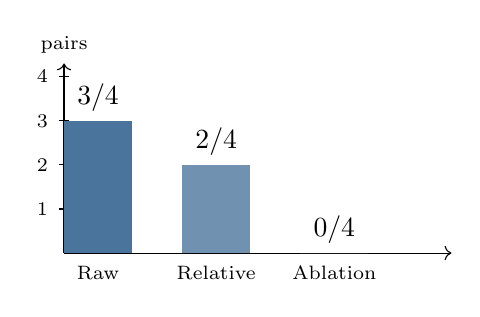
\begin{tikzpicture}[x=1.2cm,y=0.56cm]
\definecolor{diagblue}{RGB}{43,91,139}
\draw[->] (0,0) -- (4.1,0);
\draw[->] (0,0) -- (0,4.3) node[above,font=\scriptsize] {pairs};
\foreach \y in {1,2,3,4} {\draw (-0.05,\y) -- (0.05,\y) node[left,xshift=-4pt,font=\scriptsize] {\y};}
\fill[diagblue!85] (0.00,0) rectangle (0.72,3);
\node[above] at (0.36,3) {3/4};
\node[below,align=center,font=\scriptsize] at (0.36,-0.08) {Raw};
\fill[diagblue!67] (1.25,0) rectangle (1.97,2);
\node[above] at (1.61,2) {2/4};
\node[below,align=center,font=\scriptsize] at (1.61,-0.08) {Relative};
\fill[diagblue!49] (2.50,0) rectangle (3.22,0);
\node[above] at (2.86,0) {0/4};
\node[below,align=center,font=\scriptsize] at (2.86,-0.08) {Ablation};
\end{tikzpicture}
\caption{Paired mechanism discrimination in four frozen Incident 003 v3 development constructions. Raw counts only; no uncertainty bars or equivalence claim.}
\label{fig:paired}
\end{figure}

All eight responses in each stage were valid. Raw evidence yielded 7/8 exact
RCA, with 4/4 target and 3/4 twin mechanism labels correct. Relative-time
yielded 6/8 exact, 4/4 target and 2/4 twin mechanisms. Temporal ablation
yielded 4/8 exact: every target remained correct, every twin was assigned
the target's concurrency mechanism, and no pair was discriminated correctly.
The paired-mechanism sequence 3/4, 2/4, 0/4
(Figure~\ref{fig:paired}) is directionally consistent with the
preregistered development expectation that preserving temporal relations
helps distinguish the two mechanisms. It does not establish equivalence of
raw and relative time, a causal effect size for the provider, or performance
on other incidents. Four pairs and one call per case leave substantial
model-response variability unmeasured.

\section{Privacy--Utility Analysis}
\label{sec:privacy}
The measurement surface is the exact released ModelView. Exposure analysis
version 1 compares annotated raw values with the
transformed view. It reports a vector, not one privacy score. Empty
denominators are \texttt{not\_applicable}.

The vector measures literal retention, equal and unequal relations,
frequency, cross-source linkage, shape, record counts, field presence,
distinct entities, absolute time, temporal order, and exact time gaps.
Declared secrets use strict literal scanning. Other short strings use a
six-character cutoff to reduce accidental substring matches.
\begin{table}[H]
\centering
\small
\resizebox{\textwidth}{!}{%
\begin{tabular}{llrrrrrr}
\toprule
Family & Condition & Literal & Equal & Unequal & Frequency & Cross-source & Shape \\
\midrule
001 & Raw & 476/476 & 559/559 & 3459/3459 & 20/20 & 326/326 & 476/476 \\
001 & Redaction & 0/476 & 233/559 & 1709/3459 & 0/20 & 0/326 & 0/476 \\
001 & HMAC & 0/476 & 509/559 & 3459/3459 & 15/20 & 276/326 & 0/476 \\
001 & Tokenization & 0/476 & 509/559 & 3459/3459 & 15/20 & 276/326 & 0/476 \\
001 & Format-preserving & 0/476 & 509/559 & 3459/3459 & 15/20 & 276/326 & 476/476 \\
002 & Raw & 190/190 & 300/300 & 2656/2656 & 6/6 & 248/248 & 190/190 \\
002 & Redaction & 0/190 & 52/300 & 1680/2656 & 0/6 & 0/248 & 0/190 \\
002 & HMAC & 0/190 & 300/300 & 2656/2656 & 6/6 & 248/248 & 0/190 \\
002 & Tokenization & 0/190 & 300/300 & 2656/2656 & 6/6 & 248/248 & 0/190 \\
002 & Format-preserving & 0/190 & 300/300 & 2656/2656 & 6/6 & 248/248 & 190/190 \\
\bottomrule
\end{tabular}%
}
\caption{Development representation exposure for annotated identifiers. Counts are retained relationships or shapes over eligible denominators, not a privacy score.}
\label{tab:scalar-exposure}
\end{table}


All scalar transformations removed annotated direct literals in the selected
Incident 001 and 002 views. Redaction also removed measured cross-source equal
joins and collapsed many distinct values. HMAC, tokenization, and
format-preserving pseudonyms retained 276/326 cross-source equal pairs in
Incident 001 and 248/248 in Incident 002. Format-preserving pseudonyms retained
all measured shapes. HMAC and tokenization retained none of those shapes.
Record counts and annotated field presence remained intact in every scalar
condition. Unannotated timestamps also remained visible: 139/139 in Incident
001 and 478/478 in Incident 002.

The two Incident 003 roles have identical exposure vectors. Each construction
is counted once below.
\begin{center}
\small
\textbf{Incident 003 v3 development exposure, counting each construction once across two query roles. Ablation's temporal zeros mean unavailable parseable relations, not reversed time.}\par\medskip
\resizebox{\textwidth}{!}{%
\begin{tabular}{lrrrrrr}
\toprule
Condition & ID literal & Absolute & Evaluable & Order & Exact gap & Records \\
\midrule
Raw & 192/192 & 204/204 & 5004/5004 & 5004/5004 & 5004/5004 & 24/24 \\
Relative-time & 192/192 & 0/204 & 5004/5004 & 5004/5004 & 5004/5004 & 24/24 \\
Temporal ablation & 192/192 & 0/204 & 0/5004 & 0/5004 & 0/5004 & 24/24 \\
\bottomrule
\end{tabular}%
}
\end{center}

Raw retained 204/204 absolute timestamp occurrences and all 5,004 measured
order and exact-gap relations. Relative time removed the absolute literals
but retained every measured order and gap. Ablation left no parseable temporal
pair. Its zeros mean unavailable relations, not reversed order. Both temporal
conditions retained all 192 annotated non-temporal ID literals.

These measures describe visible information. They do not measure
re-identification, membership inference, auxiliary-data attacks, provider
retention, compliance, differential privacy, or legal de-identification.
No development field is classified as secret, so secret exposure is
\texttt{not\_applicable}. Synthetic tests enforce the fail-closed secret rule.

\section{Evidence-Support Methodology}
\label{sec:evidence}
A correct RCA can have weak support. DiagPriv therefore scores cited visible
evidence separately from labels. Incident 003 v3 declares essential facts for
each role. These include subject binding, deadline order, positive interval
overlap for the target, and serialized completion for the twin.

Stage 1 used \texttt{evidence-support-v4}. It required specific physical
citation paths and scored 0/8. A provider-free audit found useful log-based
proofs that did not match those paths. Version 5 therefore permits defined
alternative semantic paths. A requirement passes only when one complete path
is cited and its predicate is true on the cited ModelView records. It gives no
fuzzy, partial, or uncited credit. For positive overlap it requires
$\max(s_1,s_2)<\min(e_1,e_2)$. Opaque timestamps make time predicates
unavailable.

The Stage-1 v5 score of 3/8 is post hoc. It does not replace v4. Stages 2 and 3
froze v5 before their calls.
\begin{table}[H]
\centering
\small
\resizebox{\textwidth}{!}{%
\begin{tabular}{llrl}
\toprule
Observation & Protocol & Supported & Status \\
\midrule
Raw Stage 1 & v4 primary & 0/8 & Pre-refinement \\
Raw Stage 1 & v5 post-hoc & 3/8 & Secondary only \\
Relative-time Stage 2 & v5 prospective & 4/8 & Frozen before calls \\
Temporal ablation Stage 3 & v5 prospective & 0/8 & Frozen before calls \\
\bottomrule
\end{tabular}%
}
\caption{Incident 003 evidence support. Stage-1 v5 is a post-hoc rescore; only Stages 2 and 3 are directly comparable under prospective v5.}
\label{tab:evidence}
\end{table}

All four target responses still lacked a complete overlap proof under v5.
Stage 3 supplied no temporal essentials. Thus, label accuracy, evidence
support, and exposure remain separate outcomes.

\section{Limitations and Threats to Validity}
\label{sec:limitations}
The corpus has three synthetic families. Audits improve internal control, but
they do not show production realism. Incident 003 v3 was designed after an
earlier version exposed non-temporal shortcuts. Its audit covers known
shortcuts, not every learned cue.

Most comparisons use development data. Incident 001 has only raw validation.
Incident 002 has six constructions and a separate transport-recovery
sensitivity analysis. Incident 003 has four paired constructions and one call
per case. Its decline occurs only on twins. A concurrency category prior and
model variability remain possible. The study uses one GPT-5.6 model family.
It has no human baseline, matched validation comparison, or held-out result.

The taxonomy and component oracle are research choices. Component labels are
less stable in parts of Incidents 001 and 002. Evidence-support v5 was made
after Stage 1. Its Stage-1 use is post hoc; v4 remains the primary historical
rule.

The exposure vector measures representation, not practical attack success.
It does not test auxiliary data, membership inference, compromised HMAC keys,
provider retention, or legal compliance. Deterministic methods retain linkage
and frequency. Format preservation leaks shape. Relative time can be
reconstructed with an external anchor. Unannotated fields can remain visible.
Incorrect sensitivity labels can also expose data.

The repository does not publish provider JSONL files. It supports aggregate
reproduction, not exact response inspection. The study also excludes prompt
injection, malicious agents, poisoning, and insiders. Stronger claims require
more incidents, models, calls, human baselines, governance review, and a
preregistered held-out evaluation.

\section{Related Work}
\label{sec:related}
Clinical de-identification research shows that removal and pseudonymization
can affect downstream tasks differently
\cite{berg2020impact,bencheikhlarbi2023clinical,singh2025redactor}.
Prompt-obfuscation and task-aware anonymization work also measures privacy and
utility together
\cite{pasch2025balancing,lin2025emojiprompt,loiseau2025taueval,loiseau2026adaptive}.
DiagPriv applies this concern to linked operational evidence.

HMAC is a keyed message-authentication construction
\cite{krawczyk1997hmac}. Stable HMAC pseudonyms remove literals but keep
within-key linkage. DiagPriv's format-preserving condition keeps character
classes; it is not the cryptographic FPE defined by NIST
\cite{dworkin2016fpe}.

LLM-assisted operational RCA is established
\cite{ahmed2023recommending,chen2024automatic,wang2024rcagent,xu2025openrca}.
OpenRCA and Cloud-OpsBench provide broader operational benchmarks
\cite{xu2025openrca,wang2026cloudopsbench}. DiagPriv is smaller and synthetic.
Its focus is the evidence representation sent to the same external model.

Temporal benchmarks and contrast sets motivate controlled near-neighbor cases
\cite{chu2024timebench,gardner2020contrast}. Citation research also separates
answer quality from evidence quality
\cite{gao2023citations,zhang2024finegrained}. DiagPriv combines these ideas in
a scoped study. It does not claim to originate anonymization, RCA
benchmarking, temporal reasoning, or evidence-support scoring.

\section{Conclusion}
DiagPriv tests whether a release can hide selected literals and retain the
relations needed for RCA. The three synthetic families require linkage,
shape, or time. The paired temporal result fell from 3/4 discriminated pairs
with raw data to 2/4 with relative time and 0/4 with ablation. This small
result is consistent with a useful temporal dependency, not a general causal
estimate.

Literal removal can still expose linkage, shape, cardinality, time, and
context. The paper therefore reports RCA, evidence support, and exposure
separately. Future work needs more incidents, models, human baselines, and a
frozen held-out test before it can evaluate a task-aware selection policy.


\section*{Author Contributions}
Keshav Likhar, Harsh Mandalgi, and Mohit Chaturvedi contributed equally to
the conceptualization, methodology, investigation, validation, analysis,
and writing of this work. All authors reviewed and approved the final
manuscript.

\bibliographystyle{plain}
\bibliography{references}
\end{document}
